\section{Monday, March 3: Introduction to a simple neural network}

Main references: ISL 10.1, 10.2, 10.6, 10.7, and 10.8. I also think that ESL Chapter 11 has good context, but some of it is beyond the scope of this class. 

\subsection{A statistical motivation}

\subsubsection{GAMs, but with feature engineering?}

Last week, we discussed GAMs. These are functions where we let
$$
\hat{Y} = \hat{\beta}_0 + \hat{f}_1 (X_1) + \hat{f}_2 (X_2) + \ldots + \hat{f}_p (X_p).
$$
We let the functions $\hat{f}_j()$ be extremely non-linear functions, such as smoothing splines. Even if we let $\hat{f}_j()$ be completely non-parametric and wiggly, fitting a GAM is not too bad. The additive structure means that we can iterate through one variable at a time, and just fit a one-dimensional model of $Y - \sum_{j \neq  j^*} \hat{f}_j(X)$ on $X_{j^*}$.

But, the additive structure of the model will always introduce some bias if the true data generating mechanism is not additive! Consider image classification. Why would the image's class be determined by a sum of functions of every individual pixel? It is really the patterns between the pixels that matters. And we don't need the ability to interpret the effect of each individual pixel: this is going to be the type of data that neural networks are really good for!

We know that we could fit a GAM to the principal components of $X$. We could also manually add interaction terms. All of that would sort of help our GAM problem. But let's try to do this in an automated way.

The idea for today is that maybe we want to let:
$$
\hat{Y} = {\beta}_0 + \sum_{k=1}^K g_k(w^T X).
$$
I am getting this particular form of this equation from ESL section 11.1. This is a GAM, but it is a GAM applied to $K$ features, each of which is a linear combination of ALL of the $X$s. And we haven't yet determined the weights $w$ that will make up the linear combinations. In projection pursuit regression (ESL, 11.1), the $g_k()$ are smoothers, as in additive models. Today, we will have them be something simpler. 

As noted in ESL, project pursuit regression never became widely used. This is because, at the time of its introduction, you would need really powerful computers to actually fit the model. However, the reason that it is exciting for us is that it was a completely statistical motivation for a topic that was simultaneously becoming popular in the field of AI. We will discuss the AI motivation later. 


%When we classify an image, we know that there is important information about the image stored in the pixels. But each pixel on its own is useless! We need a way to learn intermediate concepts or features that will actually help us classify the image. The difference between what we are doing today and what we did with PCA regression is that (1) we learn the new features with the help of $Y$ (PCA did not look at $Y$) and (2) the learned features are not simply linear combinations of the original features (with PCA they were!).  Check out ESL Chapter 11.1 on Projection Pursuit regression. This was a way in which statisticians sort of came up with the Neural network model in a way that was totally separate from the artificial intelligence perspective of

\subsubsection{The neural network model}

ISL introduces its first neural network model on page 404. The idea is that we will let $\hat{Y} = \hat{f}(X)$, where $\hat{f}(X)$ must come from a class of functions that can be written as: 
\begin{align}
\nonumber
{f}(X) &= {\beta}_0 + \sum_{k=1}^K {\beta}_k h_k(X)  \\
\label{eq_NN}
&=  {\beta}_0 + \sum_{k=1}^K {\beta}_k g\left(w_{k0} + \sum_{j=1}^p w_{kj} X_j \right). 
\end{align}
The function $g()$ is a non-linear activation function. The idea is that we model $Y$ as a linear combination of $K$ ``hidden units" or ``activations". $K$ is a parameter that we get to pick. Each of these is a non-linear transformation of a simple linear combination of the $X$ variables. Note that if we chose $g()$ to be a linear function, this would just collapse down into a linear model with no interaction terms. 

So ... this is our neural network! We need to use our training data to come up with estimates for $\beta_0, \beta_1, ..., \beta_K$ and $w_{k0}, \ldots, w_{kp}$ for $k=1,\ldots, K$. This is a total of $(K+1)+(p+1)*K = (p+2)\times K+1$ parameters. We want to come up with guesses such that $Y \approx \hat{f}(X)$, hopefully on both out training data but also on unseen test data. 

Because of the fact that there are so many parameters in \eqref{eq_NN}, we often draw this model as a picture so as to keep track of everything. The picture is shown in Figure~\ref{fig_nn}. The idea is that every line in the picture corresponds to a parameter that we learn. Once we have drawn this as a picture, we can call the setup of our model the ``architecture". The architecture is up to us! If we wanted to have hidden node $A_1$ not connect to $X_1$, that would be totally fine: we would just have one less arrow in our picture and one less parameter to estimate. 

There is one note in Figure~\ref{fig_nn} that is not reflected in \eqref{eq_NN}. In \eqref{eq_NN}, I was imagining a regression problem: so once we take our linear combination of linear combinations, we have $\hat{Y} = \hat{f}(X)$. If we are doing classification, we might want a final step where we convert the output of our network into a probability (using a sigmoid or softmax function), and then maybe convert it to a discrete prediction. Multi-class classification is seamless: we just have one output node per class, and we later convert to probabilities with a softmax function. 

\begin{figure}[h]
\centering
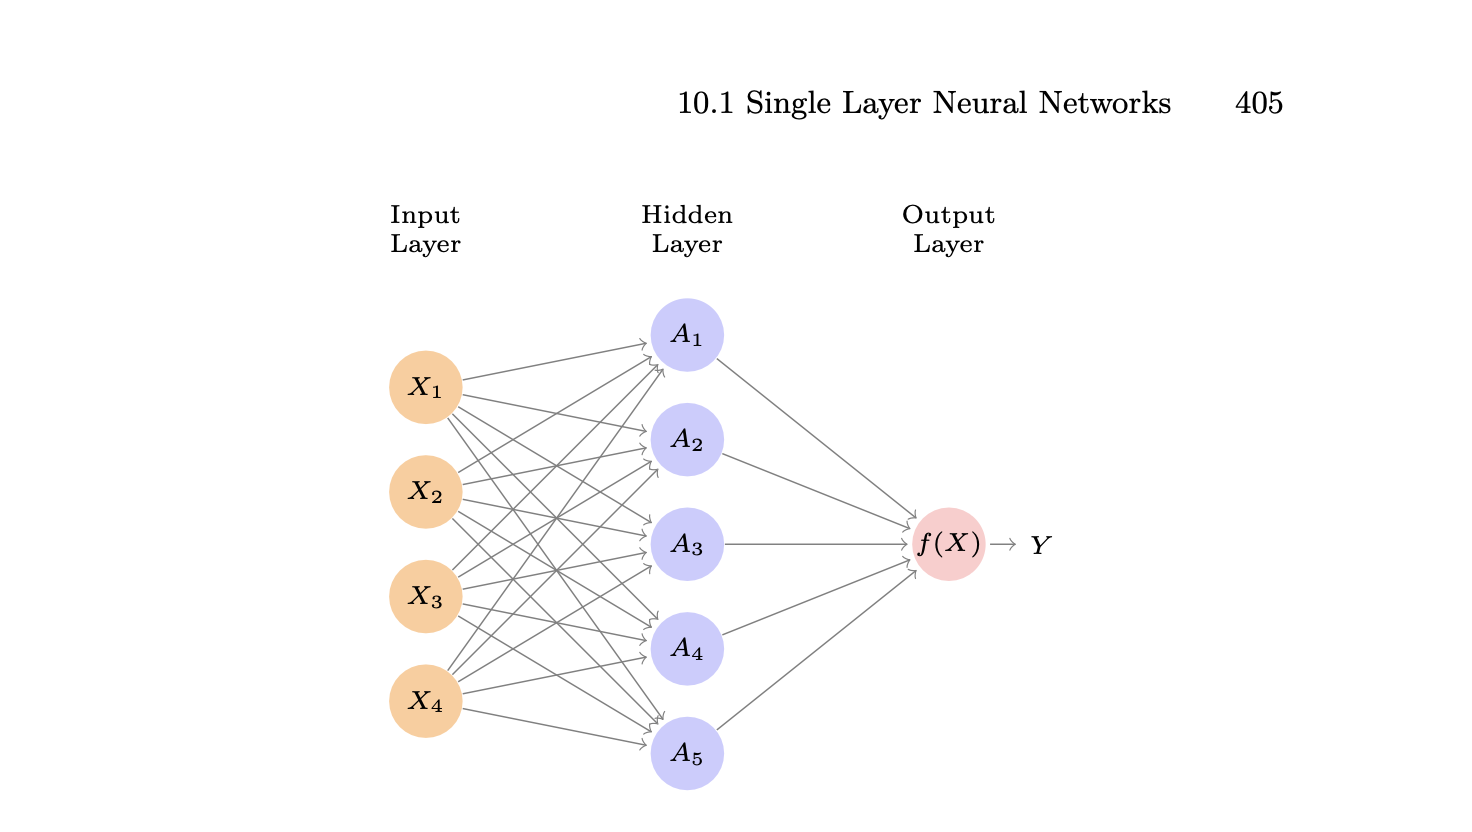
\includegraphics[width=0.8\textwidth]{442_lecs/nn.png}
\caption{A visualization of \eqref{eq_NN}. The arrows between the inputs $X$ and the hidden later each represent a parameter $w_{kj}$, where the $k$ tells us which hidden layer we connect to and the $j$ tells us which input variable to connect to. Sometimes we draw an extra input layer node to represent the intercept. The arrows from the hidden layer to the prediction layer are the parameters $\beta_k$. All of these parameters must get estimated.}
\label{fig_nn}
\end{figure}

While we won't be able to fit models like the one shown in Figure~\ref{fig_nn} directly with least squares, we will be able to fit it by optimizing over a loss function: something that you all have already seen many times! So ... a neural network really isn'y all that different from a linear model! This is a very statistical perspective on neural networks.

\subsubsection{Deep learning}

The really key idea in Figure~\ref{fig_nn} is that: \textbf{linear combinations of non-linear transformations of linear combinations} can be arbitrarily complicated and wiggly! In fact, there is a theorem that says that any continuous function $f()$ can be expressed in the form \eqref{eq_NN} as long as $g()$ is non-polynomial and $K$ is big enough. Another idea, if we don't want to make $K$ huge, is to add more layers! And more levels of non-linearity! This is shown in Figure~\ref{fig_deep}, which is also taken from ISL. 

The idea of approximating really complicated functions with these networks has really taken off in the field of deep learning! Models like the one in Figure~\ref{fig_deep} have become very state of the art in image classification, computer vision, LLMs, and basically any other big-tech application that you can possibly think of. Whatever big data you see out there in the real world- it is probably making use of deep neural networks! It almost makes me feel like there is no need to teach the other methods that we have been discussing or will be discussing in this class. But only almost! Deep neural networks are not appropriate for every circumstance, and they certainly have a lot of downsides!  

\begin{figure}[h]
\centering
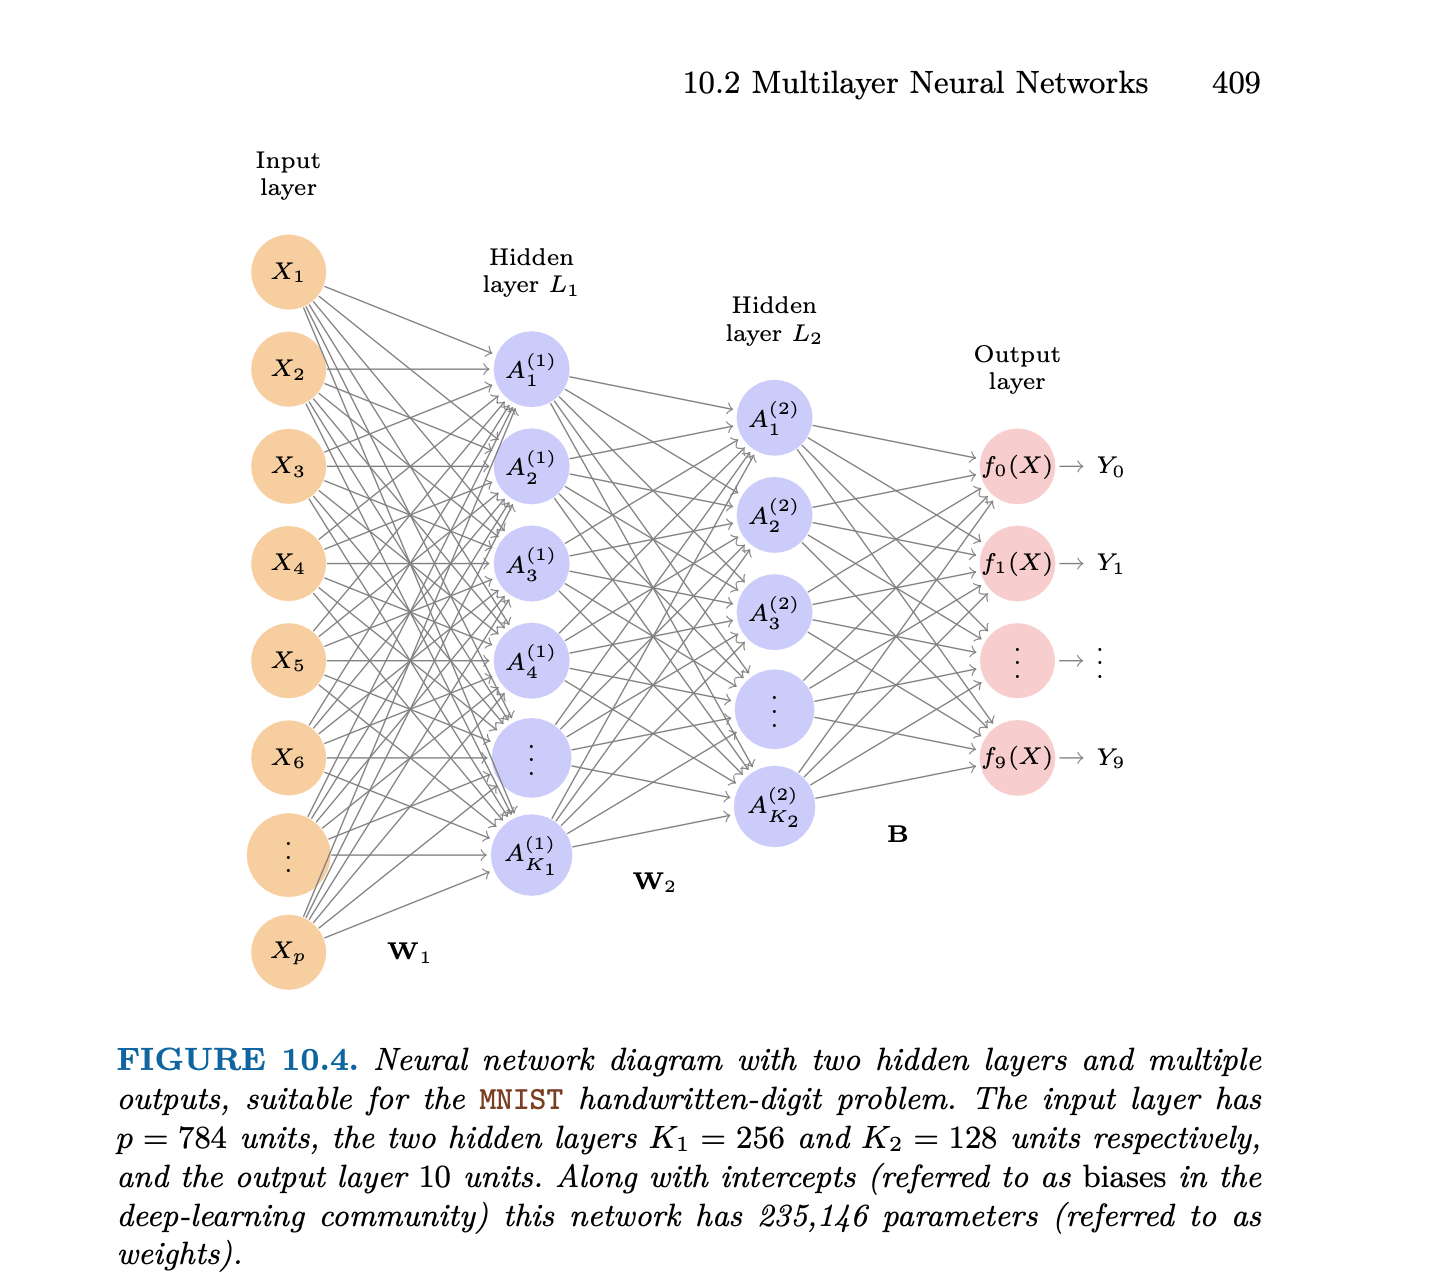
\includegraphics[width=0.8\textwidth]{442_lecs/deep.png}
\caption{A multilayer neural net. Note that here we have multiple outputs $Y$ because this is for a categorical output with 10 categories. We represent this as a vector of length 10, where $Y_k=1$ if $Y=k$ and $Y_k=0$ otherwise.}
\label{fig_deep}
\end{figure} 

\subsection{Historical context and a less statistical motivation}

When neural networks were first developed in the 1940s, there was a biological interpretation. Scientists wanted to model the living brain! An early reference is McCulloch and Pitts (1943). 

The nodes in the hidden layer are supposed to represent neurons. A neuron only fires if the amount of signal being passed into it exceeds a certain threshold. So, the activation function $g()$ was typically a step function: either the node (neuron) is turned on, or turned off. However, the step function was later replaced with differentiable alternatives for the purposes of actually fitting the model. But, the idea that the activation function should often be near 0 until it eventually gets ``activated" or ``fires" remained. 

Do you think that neural networks work well because they model the human brain (which works well), or do you think they work well because they are very expressive linear models that do automatic feature engineering? It is up to you to decide on your interpretation! I think the latter, but I also do not know much about the real human brain! 

A few more historical notes:
\begin{itemize}
\item The ideas of neural networks are so old and were developed independently by different fields!
\item But ... when did they really take off?
\item Up until 2010 or so, they were not popular in computer vision. Only Yann LeCun and Geoff Hinton were really pursuing these. After some students of Geoff Hinton won an ImageNet competition (used a neural network for an image classification task and got the best performance), then people started to pay attention.
\item By the way, my history	 knowledge was really rusty and anecdotal. I found this slide deck from a course at Univ. Wisconsin \url{https://sebastianraschka.com/pdf/lecture-notes/stat479ss19/L02_dl-history_slides.pdf} and I liked the way the material was presented: he has screenshots from a lot of cool books. Check these out and check out the related sources if you want to know more!
\item Things I learned: the ReLU activation function was an idea of Hinton+coauthor, and it was in 2010. And this change in activation function must have been a huge difference maker! 
\item You can also check out Section 1.2 of the free deep learning book: \url{https://www.deeplearningbook.org}. 
\end{itemize}



\subsection{What do I pick for my activation function $g()$?}
\begin{itemize}
\item In projection pursuit regression, the idea was that this could be a smoothing spline or something! But projection pursuit regression was always going to have like $K=5$ and one hidden layer. If we want to do BIG neural networks, we need something simple. And hopefully differentiable, because we will fit with gradient descent. 
\item From the ``neurons in the brain" view of neural networks, a 0/1 step function made sense. A neuron is either turned on or turned off. But, since a step function is not differentiable, the sigmoid/logistic: $g(z) = \frac{1}{1+e^{-z}}$ was a nice alternative. Or tanh. 
\item But, nowadays, a really common one is: $g(z) = max(0,z)$. This is called the ReLU. This keeps the motivation of a neuron being ``turned on" vs. ``turned off," but now allows really strong signals to be carried forward by having larger magnitude. One issue with this activation function is the ``dead ReLU" problem, which we will discuss. 
\end{itemize}





\subsection{Themes}

People have the tendency to treat neural networks and deep learning as magical! I hope to convince you that these are not magical, and that they in fact relate to many things that you have already seen in this class: e.g. feature engineering, basis expansion. And I hope you can start to see how neural networks relate a bit to what I talked about on the very first day of class: the biggest difference between modern machine learning and classical statistics has to do with ``how much is pre-specified". Neural network relates to feature engineering or basis expansions, but the form of the new features or the basis functions was not pre-specified.

Because NNs are not so different than everything else we can see in this class, we can discuss our favorite themes. 
\begin{itemize}
\item Bias:
\begin{itemize}
\item  We can approximate ANY continuous function $f$ with a neural network with one hidden layer and a non-polynomial activation function. We might need a really huge (but finite) value of $K$. But still! This is so cool. It means that we are not limited by modeling assumptions for a neural network: we should be able to model any true $f$ really well.
\item One note: this theorem	 says that any continuous function $f$ can be expressed using a picture like Figure~\ref{fig_nn} and certain values of the weights. It does not say that we will be able to estimate the weights from our training data! 
\item But still. Neural networks have really low bias! No bias if we use enough layers or nodes. 
\item They work really well!
\end{itemize}
\item Variance
\begin{itemize}
\item We know that variance depends on degrees of freedom, which is the effective number of parameters that we are estimating. If we make a lot of hidden layers, or if we make $K$ really big, then surely we will have more parameters than we do training observations $n$. Isn't this really bad for variance? Won't we memorize our training set and overfit?
\item Short answer: statisticians were very skeptical of deep learning for these reasons for many years. Over-parameterized models should score poorly for variance! And they definitely do when you don't have a really big value of $n$. 
\item We should regularize to help keep the variance under control. More on this when we discuss double descent! We should use a validation set to stop training before we overfit.
\item But sometimes, when you have enough data, NNs perform really well on test sets, even though they are over-parameterized. This also isn't magic: we need to distinguish between number of parameters and number of effective parameters
\end{itemize}
\item Interpretability
\begin{itemize}
\item This is our first true black-box model. It is really hard to understand where the predictions of a neural network model are coming from!
\item Do not pick deep learning if you have a scientific application where you need to interpret and explain your results!
\item Since the model itself is a black-box, we will need to use clever explainability techniques on top of the model to try to understand what is going on: this is a hot area of research that we will discuss after spring break.  
\end{itemize}
\item Usability (is the method ``off the shelf")?
\begin{itemize}
\item Neural networks tend to require a lot more tuning than something like a random forest. They are NOT very ``off-the-shelf". This is a reason why they took a while to become popular. They were hiding in the background for many years before deep learning really took off. 
 \item Evidence: I will not make you do a HW problem where you actually use neural nets, because the R packages are finicky! 
\item There is flexibility, which is nice: you can modify the architecture really to your liking. If you know what you are doing, this is great! But this flexibility does make it harder to make all-purpose, useable software. 
\end{itemize}
\item Computational efficiency	
\begin{itemize}
\item We are going to actually go over gradient descent and backpropogation on Thursday! So you will learn more about fitting. 
\item We need to use a slow iterative algorithm to fit: and we always need to be worried that maybe we did not converge in our fitting! 
\item However, there is also something very parallel and distributed about our computations, which makes huge deep neural networks actually feasible to fit. 
\end{itemize}
\end{itemize}




